\documentclass{article}

\usepackage{geometry}
\usepackage{longtable}
\usepackage[dvipsnames,table]{xcolor}
\usepackage{fancyhdr}
\usepackage{xcolor}
\usepackage{graphicx}
\usepackage{hyperref}
\usepackage{float}
\usepackage{listings}
\usepackage{amssymb}
\usepackage{amsmath}
\usepackage{enumitem}
\usepackage{parskip}

% Choose paper size
\geometry{letterpaper, top=25.4mm, bottom=25.4mm, left=25.4mm, right=25.4mm}
%\geometry{a4paper, top=25.4mm, bottom=25.4mm, left=25.4mm, right=25.4mm}

\color{black}
\fancyhf{}
\renewcommand{\headrulewidth}{1pt}
\renewcommand{\footrulewidth}{1pt}

% Define standard IPF color palette
\definecolor{soft-sky-blue}{HTML}{B7DAEB}
\definecolor{orange}{HTML}{FF6633}
\definecolor{cool-grey}{HTML}{91A1B0}
\definecolor{black}{HTML}{000000}
\definecolor{space-blue}{HTML}{003366}
\definecolor{pigeon-blue}{HTML}{5F8396}
\definecolor{sage-green}{HTML}{95A077}
\definecolor{fire-yellow}{HTML}{F9A651}
\definecolor{apple-red}{HTML}{CC4200}
\definecolor{crockadile-green}{HTML}{718944}
\definecolor{slate-grey}{HTML}{607587}
\definecolor{fog-grey}{HTML}{E5E6E9}

% Define certification colors
\definecolor{cert-level-0}{HTML}{CC4200} % apple-red
\definecolor{cert-level-1}{HTML}{FF6633} % orange
\definecolor{cert-level-2}{HTML}{F9A651} % fire-yellow
\definecolor{cert-level-3}{HTML}{B7DAEB} % soft-sky-blue
\definecolor{cert-level-4}{HTML}{5F8396} % pigeon-blue
\definecolor{cert-level-5}{HTML}{718944} % sage-green

\hypersetup{hidelinks}
\pagestyle{fancy}
\pagenumbering{arabic}

\title{
\includegraphics[width=8cm] {images/Rocksavage_Tech_RGB_300.png}\vspace{50pt}
\vspace{10pt} \\
\textbf{Gpio \\
  Product User Guide} \\
{\small{\textcolor{slate-grey}{rocksavagetech.chiselWare.Gpio}}} \\
\vspace{20pt} IPF certified to level:
\textbf{\textcolor{cert-level-0}{0} }of 5 \\
\vspace{5pt}
\includegraphics[width=4cm] {images/uncertified.png}
}

\author{Abdelrahman Abbas, Ahmed Elmenshawi, Nick Allison, Jimmy Bright}

\fancyhead[L]{Gpio Users Guide}
\fancyhead[R]{\leftmark}
\fancyfoot[C]{Rocksavage Technology, Inc.~\copyright~2023}
\fancyfoot[R]{Page \thepage}

\begin{document}

\maketitle
\newpage
\tableofcontents

\include{./errata}
% chktex-file 44
\section{Port Descriptions}

\subsection{Gpio Interface}

The ports for \textbf{Gpio} are shown below in 
Table 1. The width of several ports is controlled 
by the following input parameters:

\textit{dataWidth} is the width of the gpioInput, gpioOutput, and gpioOutputEnable ports in bits
 
\renewcommand*{\arraystretch}{1.4}
\begin{longtable}[H]{
  | p{0.20\textwidth}
  | p{0.20\textwidth}
  | p{0.12\textwidth}
  | p{0.43\textwidth} |
  }
  \hline
  \textbf{Port Name} &   
  \textbf{Width} &   
  \textbf{Direction} &   
  \textbf{Description} \\ \hline \hline

  gpioInput &       
  \textit{dataWidth} & 
  Input &       
  Data to be sent to the Gpio\\ \hline

  gpioOutput &        
  \textit{dataWidth} & 
  Output &       
  Data to be recieved from the Gpio \\ \hline

  gpioOutputEnable &      
  \textit{dataWidth} & 
  Output &     
  Enable data to be recieved from the Gpio \\ \hline

  irqOutput &      
  1 & 
  Output &     
  Sent when interrupt is triggered on the Gpio \\ \hline
 
 
  \caption{Gpio Ports Descriptions}\label{table:ports}
\end{longtable}

\subsection{Apb3 Interface}
The \textbf{Apb3 Interface} is a regular Apb3 Slave Interface. All signals supported are shown below in 
Table 2. See the \textit{AMBA Apb Protocol Specifications} for a complete description of the signals. The width of several ports is controlled 
by the following input parameters:

\begin{itemize}[noitemsep]
  \item \textit{dataWidth} is the width of PWDATA and PRDATA in bits
  \item \textit{addrWidth} is the width of PADDR in bits
\end{itemize}
 
\renewcommand*{\arraystretch}{1.4}
\begin{longtable}[H]{
  | p{0.20\textwidth}
  | p{0.20\textwidth}
  | p{0.12\textwidth}
  | p{0.43\textwidth} |
  }
  \hline
  \textbf{Port Name} &   
  \textbf{Width} &   
  \textbf{Direction} &   
  \textbf{Description} \\ \hline \hline

  PCLK &       
  1 &       
  Input &       
  Positive edge clock \\ \hline

  PRESETN &       
  1 &       
  Input &       
  Active low reset \\ \hline

  PSEL &       
  1 & 
  Input &       
  Indicates slave is selected and a data transfer is required \\ \hline

  PENABLE &        
  1 & 
  Input &       
  Indicates second cycle of Apb transfer \\ \hline

  PWRITE &        
  1 & 
  Input &       
  Indicates write access when HIGH and read access when LOW\\ \hline

  PADDR &      
  \textit{addrWidth} & 
  Input &     
  Address bus \\ \hline

  PWDATA &      
  \textit{dataWidth} & 
  Input &     
  Write data bus driven when PWRITE is HIGH\\ \hline

  PRDATA &      
  \textit{dataWidth} & 
  Output &     
  Read data bus driven when PWRITE is LOW\\ \hline
 
  PREADY &        
  1 & 
  Output &       
  Transfer ready \\ \hline

  PSLVERR &        
  1 & 
  Output &       
  Transfer error \\ \hline

  \caption{Apb Ports Descriptions}\label{table:interface}
\end{longtable}


% chktex-file 44

\section{Parameter Descriptions}

The parameters for \textbf{Gpio} are shown below in
Table 3.

\renewcommand*{\arraystretch}{1.4}
\begingroup
\small
\rowcolors{2}{gray!30}{gray!10} % Alternating colors start from the second row
\arrayrulecolor{gray!50}
\begin{longtable}[H]{
    | p{0.25\textwidth}
    | p{0.10\textwidth}
    | p{0.05\textwidth}
    | p{0.05\textwidth}
    | p{0.47\textwidth} |
  }
  \hline
  \rowcolor{dark-gray}

  \textcolor{white}{\textbf{Name}} &
  \textcolor{white}{\textbf{Type}} &
  \textcolor{white}{\textbf{Min}} &
  \textcolor{white}{\textbf{Max}} &
  \textcolor{white}{\textbf{Description}} \\ \hline
  \endfirsthead

  \textcolor{white}{\textbf{Name}} &
  \textcolor{white}{\textbf{Type}} &
  \textcolor{white}{\textbf{Min}} &
  \textcolor{white}{\textbf{Max}} &
  \textcolor{white}{\textbf{Description}}            \\ \hline
  \endhead


  \endfoot

  dataWidth   &
  Int       &
  1         &
  $\leq$ 32          &
  The data width of Gpio ports, PWDATA, and PRDATA. Can be 8, 6, or 32 bits wide \\ \hline

  addrWidth     &
  Int           &
  1             &
  $\leq$ 32       &
  The Apb address bus width  \\ \hline

\end{longtable}
\captionsetup{aboveskip=0pt}
\captionof{table}{Parameter Descriptions}\label{table:params}
\endgroup

The Gpio is instantiated into a design as follows:

\begin{lstlisting}[language=Scala]

  // Valid Gpio Instantiation Example
  val myGpio = new Gpio(
    dataWidth = 32, 
    addrWidth = 32 ) 

  \end{lstlisting}

\section{Operating Modes}

\subsection{Introduction}
The Gpio core supports bidirectional IO pads, and each IO can be programmed to operate in 
push-pull or open drain mode, as defined by te MODE register.

Note: IO Pads are not implemented within the Gpio core - this is the responsiblity of the designer

\subsection{Push-Pull Mode}
In this mode, each bit of gpioOutput is driven from the internal OUTPUT register. The gpioOutputEnable bus is controlled via the DIRECTION register and 
specifies whether or not the pin will allow the IO Pad to see the corresponding OUTPUT data.

\begin{figure}[h]
    \centering
    \includegraphics[width=0.4\textwidth]{images/ppl.png}
    \caption{Push Pull Mode}
  \end{figure}

\subsection{Open Drain Mode}
In this mode, each bit of gpioOutput is driven low when the corresponding OUTPUT register bit is low and corresponding DIRECTION register bit is high. 
This allows for multiple devices to pull the line low without conflicting high/low states on the output pin.

\begin{figure}[h]
    \centering
    \includegraphics[width=0.4\textwidth]{images/od.drawio.png}
    \caption{Open Drain Mode}
  \end{figure}

\section{Theory of Operations}

\subsection{Introduction}
The \textbf{GPIO} module is configurable with parameters for setting data and address widths. It interfaces with the CPU via the APB3 bus. The signals \textbf{gpioInput}, \textbf{gpioOutput} and \textbf{gpioOutputEnable} are designed to interface with external hardware, such as a tri-state buffer, to facilitate bi-directional communication on physical pins.

\begin{figure}[h]
  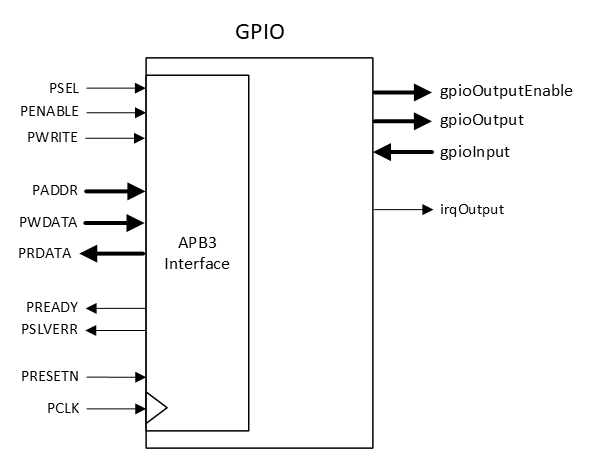
\includegraphics[width=0.90\textwidth]{images/block-diagram-gpio.png}
  \caption{GPIO Block Diagram}\label{fig:block-diagram}
\end{figure}

% It features the following status flags which are described in
% Table~\ref{table:ports}.

% \begin{itemize}[noitemsep]
%   \item{empty}
%   \item{full}
%   \item{almostEmpty}
%   \item{almostFull}
% \end{itemize}

% When \textit{push} is asserted, the data on the \textit{dataIn} port is enqued
% on the next rising edge of \textit{clock}. When \textit{pop} is asserted, the
% top of the FIFO is dequed and immediately available on the \textit{dataOut}
% port. Pop and Push operations can be simulataneous.

% There are two error conditions which produce the following effects:
% \begin{itemize}
%   \item{When \textit{pop} is asserted and the FIFO is empty (\textit{empty} is
%         active), \textit{dataOut} will contain the last valid data held in
%         the FIFO.}
%   \item{When \textit{push} is asserted and the FIFO is full (\textit{full} is
%         active), \textit{dataIn} will be ignored and not enqued.}
% \end{itemize}

% The \textit{almostEmpty} and \textit{almostFull} flags allow for additional
% feedback to the system that is useful for optimizing data flow control. The
% levels of these flags can be programmed dynamically through the
% \textit{almostEmptyLevel} and \textit{almostFullLevel} ports.

\newpage
\subsection{Interface Timing}

GPIO has a synchronous APB3 interface, and a GPIO interface. The timing diagram shown below
in Figure~\ref{fig:timing} represents an instantiation with the following
parameters.

\begin{lstlisting}[language=Scala]
val myGPIO = new GPIO(
  dataWidth = 16, 
  addrWidth = 16 ) 
\end{lstlisting}

\begin{figure}[h]
  \includegraphics[width=\textwidth]{images/GPIO-timing.png}
  \caption{Timing Diagram}\label{fig:timing}
\end{figure}

This shows the operation of the basic read/write register operations following the APB protocol. Registers DIRECTION, MODE, and OUTPUT are
written to, while register INPUT is read from.

The \textit{gpioOutputEnable} port is driven to a value of 0x000F after 0x000F is written to the DIRECTION register 
at address 0x00. Next, the MODE register at address 0x06 is written a value of 0x0009. The \textit{gpioOutput} port 
then has a value of 0x0009 because of the open-drain mode operation. 

The OUTPUT register is then written a value of 0x0006 at address 0x02. \textit{gpioOutput} takes on a value of 0x000F
since the MSB and LSB are operating on open-drain mode, and the middle two bits are operating on push-pull mode. 

The INPUT register is read from at address 0x04, which has a value of 0x0070 since \textit{gpioInput} has a value fo 0x0070.
On the final transaction, PSLVERR goes high because an invalid address is written to.

% nested include
% chktex-file 44
\subsection{Register Interface}
 
When programming registers, each register starts on a byte address, and the last bits it would take up in its final byte based on its size are unused. To find the size in bytes for any register, divide by the register size, and round up to the nearest whole number. For example, a 32-bit register would take up 4 bytes, and a 1-bit register would take up 1 byte.
 
\begin{longtable}[H]{
  | p{0.27\textwidth}
  | p{0.18\textwidth}
  | p{0.50\textwidth} |
  }
  \hline
  \textbf{Name} &   
  \textbf{Size (Bits)} &   
  \textbf{Description} \\ \hline \hline

  DIRECTION  &   
  dataWidth &   
  DESC TODO \\ \hline

  OUTPUT &   
  dataWidth &   
  DESC TODO \\ \hline

  INPUT &   
  dataWidth &   
  DESC TODO \\ \hline

  MODE &   
  dataWidth &   
  DESC TODO \\ \hline

  ATOMIC\_OPERATION &   
  4 &   
  DESC TODO \\ \hline

  ATOMIC\_MASK &   
  p.dataWidth &   
  DESC TODO \\ \hline

  ATOMIC\_SET &   
  1 &   
  DESC TODO \\ \hline

  VIRTUAL\_PORT\_MAP &   
  sizeOfVirtualPorts &   
  DESC TODO \\ \hline

  VIRTUAL\_PORT\_OUTPUT &   
  numVirtualPorts &   
  DESC TODO \\ \hline

  VIRTUAL\_PORT\_ENABLE &   
  1 &   
  DESC TODO \\ \hline

  TRIGGER\_TYPE &   
  dataWidth &   
  DESC TODO \\ \hline
  
  TRIGGER\_LO &   
  dataWidth &   
  DESC TODO \\ \hline
  
  TRIGGER\_HI &   
  dataWidth &   
  DESC TODO \\ \hline
  
  TRIGGER\_STATUS &   
  dataWidth &   
  DESC TODO \\ \hline
  
  IRQ\_ENABLE &   
  dataWidth &   
  DESC TODO \\ \hline

\end{longtable}

  \newpage

  \subsubsection{Register Operation}
  \paragraph{DIRECTION:}
  DIRECTION is a \textit{dataWidth} bits wide active-high read/write register. This register controls the 
  output enable bus \textit{gpioOutputEnable}. Operation can be seen in Table
  \begin{table}[h]
    \centering
    \begin{tabular}{|c|c|}
        \hline
        \textbf{DIRECTION[n]} & \textbf{Direction} \\ \hline
        0 & Input \\ \hline
        1 & Output \\ \hline
    \end{tabular}
    \caption{DIRECTION Register}
\end{table}

\paragraph{OUTPUT:}
OUTPUT is a \textit{dataWidth} bits wide read/write register. This register controls the 
output bus \textit{gpioOutput}. Writing a '0' drives the pad low in both modes of operation. Writing a '1' 
drives the pad high in push-pull mode, or Hi-Z in open-drain mode. 

\paragraph{INPUT:}
INPUT is a \textit{dataWidth} bits wide read-only register. This register is written to from the 
input bus \textit{gpioInput}. On the rising edge of the APB3 Bus Clock (PCLK), input data from \textit{gpioInput} 
is synchronized using two flops and stored in the INPUT register. From there, it may be read via the APB3 Bus Interface
through PRDATA. 

\paragraph{MODE:}
MODE is a \textit{dataWidth} bits wide read/write register. This register sets the operating mode for each bit
of the \textit{gpioOutput} and \textit{gpioOutputEnable} busses as either push-pull or open drain mode. Operation can be seen in Table
\begin{table}[h]
  \centering
  \begin{tabular}{|c|c|}
      \hline
      \textbf{MODE[n]} & \textbf{Operating Mode} \\ \hline
      0 & Push-Pull \\ \hline
      1 & Open Drain\\ \hline
  \end{tabular}
  \caption{MODE Register}
\end{table}

% truth table for atomic set from atomic operation
% p3_p2_p1_p0 ->
% 
%         Out
%         0  1
%  Mask 0 p1 p0
%       1 p3 p2
\paragraph{ATOMIC\_OPERATION:}
ATOMIC\_OPERATION is a 4 bits wide read/write register. This register sets the atomic operation to be performed on the
of gpio registers. The operation is performed on the \textit{OUTPUT} register and is performed atomically.

\paragraph{ATOMIC\_MASK:}
ATOMIC\_MASK is a \textit{dataWidth} bits wide read/write register. This register is used to mask the atomic operation on the \textit{OUTPUT} register. 
The specific operation used is determined by the ATOMIC\_OPERATION register seen in the above table.

\paragraph{ATOMIC\_SET:}
ATOMIC\_SET is a 1 bit wide read/write register. This register is used to trigger the atomic operation on the \textit{OUTPUT} register. 
When ATOMIC\_SET is written to, the operation specified in ATOMIC\_OPERATION is performed on the \textit{OUTPUT} register.

\paragraph{VIRTUAL\_PORT\_MAP:}
VIRTUAL\_PORT\_MAP is a \textit{sizeOfVirtualPorts} bits wide read/write register. This register maps the virtual ports to the physical pins.
Each bit in the register corresponds to a virtual port, and the value of the bit determines which physical pin the virtual port is mapped to 
according to the following table by default:
\begin{table}[h]
  \centering
  \begin{tabular}{|c|c|}
      \hline
      \textbf{VIRTUAL\_PORT\_MAP[n]} & \textbf{Physical Pin} \\ \hline
      0 & Pin 0 \\ \hline
      1 & Pin 0 \\ \hline
      2 & Pin 0 \\ \hline
      3 & Pin 0 \\ \hline
      4 & Pin 0 \\ \hline
      5 & Pin 0 \\ \hline
      6 & Pin 0 \\ \hline
      7 & Pin 0 \\ \hline
  \end{tabular}
  \caption{VIRTUAL\_PORT\_MAP Register}
\end{table}

\paragraph{VIRTUAL\_PORT\_OUTPUT:}
VIRTUAL\_PORT\_OUTPUT is a \textit{numVirtualPorts} bits wide read/write register. This register sets the output value of the virtual ports.
Each bit in the register corresponds to a virtual port, and the value of the bit determines the output value of the virtual port.

\paragraph{VIRTUAL\_PORT\_ENABLE:}
VIRTUAL\_PORT\_ENABLE is a 1 bit wide read/write register. This register enables the virtual ports. When VIRTUAL\_PORT\_ENABLE is set to '1', the virtual ports are enabled.
When VIRTUAL\_PORT\_ENABLE is set to '0', the virtual ports are disabled.

\paragraph{TRIGGER\_TYPE:}
TRIGGER\_TYPE is a \textit{dataWidth} bits wide read/write register. This register configures whether \textit{gpioInput} is a level or edge sensitive
interrupt trigger as seen below:
\begin{table}[h]
  \centering
  \begin{tabular}{|c|c|}
      \hline
      \textbf{TRIGGER\_TYPE[n]} & \textbf{Type} \\ \hline
      0 & Level \\ \hline
      1 & Edge \\ \hline
  \end{tabular}
  \caption{TRIGGER\_TYPE Register}
\end{table}

\newpage

\paragraph{TRIGGER\_LO:}
TRIGGER\_LO is a \textit{dataWidth} bits wide read/write register. This register configures whether the interrupt is triggered on a level low, or a falling edge, 
of \textit{gpioInput} depending on how TRIGGER\_TYPE is set. Operation can be see in Table:
\begin{table}[h]
  \centering
  \begin{tabular}{|c|c|c|}
      \hline
      \textbf{TRIGGER\_LO[n]} & \textbf{Level Trigger} & \textbf{Edge Trigger} \\ \hline
      0 & No Trigger when Low & No Trigger on Falling Edge\\ \hline
      1 & Trigger when Low & Trigger on Falling Edge\\ \hline
  \end{tabular}
  \caption{TRIGGER\_LO Register}
\end{table}

\paragraph{TRIGGER\_HI:}
TRIGGER\_HI is a \textit{dataWidth} bits wide read/write register. This register configures whether the interrupt is triggered on a level high, or a rising edge, 
of \textit{gpioInput} depending on how TRIGGER\_TYPE is set. Operation can be see in Table:
\begin{table}[h]
  \centering
  \begin{tabular}{|c|c|c|}
      \hline
      \textbf{TRIGGER\_HI[n]} & \textbf{Level Trigger} & \textbf{Edge Trigger} \\ \hline
      0 & No Trigger when High & No Trigger on Rising Edge\\ \hline
      1 & Trigger when High & Trigger on Rising Edge\\ \hline
  \end{tabular}
  \caption{TRIGGER\_HI Register}
\end{table}

\paragraph{TRIGGER\_STATUS:}
TRIGGER\_STATUS is a \textit{dataWidth} bits wide read/write register. This register sets a corresponding bit to '1' if a trigger condition is met on
the corresponding \textit{gpioInput[n]} according to the settings of TRIGGER\_TYPE, TRIGGER\_LO, and TRIGGER\_HI.
\newline
\newline
TRIGGER\_STATUS may be read on the PRDATA bus to determine if a trigger condition has occurred. Writing a '1' to TRIGGER\_STATUS[n] will clear the 
status of the corresponding bit. If a new trigger is detected simulatenously during this write, the TRIGGER\_STATUS[n] will remain set.
\begin{table}[h]
  \centering
  \begin{tabular}{|c|c|}
      \hline
      \textbf{TRIGGER\_STATUS[n]} & \textbf{Status} \\ \hline
      0 & No Trigger Detected \\ \hline
      1 & Trigger Detected\\ \hline
  \end{tabular}
  \caption{TRIGGER\_STATUS Register}
\end{table}

\newpage
\paragraph{IRQ\_ENABLE:}
IRQ\_ENABLE is a \textit{dataWidth} bits wide read/write register. This register determines if the \textit{irqOutput} pin is asserted when a trigger condition
occurs on the corresponding TRIGGER\_STATUS[n]. IRQ\_ENABLE is responsible for enabling interrupt generation from the Gpio core.
\begin{table}[h]
  \centering
  \begin{tabular}{|c|c|}
      \hline
      \textbf{IRQ\_ENABLE[n]} & \textbf{Definition} \\ \hline
      0 & Disable IRQ Generation\\ \hline
      1 & Enable IRQ Generation \\ \hline
  \end{tabular}
  \caption{IRQ\_ENABLE Register}
\end{table}

\newpage

\subsubsection{Register Addresses:}
\paragraph{dataWidth: 8}
\begin{table}[h]
  \centering
  \begin{tabular}{|c|c|c|}
      \hline
      \textbf{Register Name} & \textbf{Address Start} & \textbf{Address End} \\ \hline
      DIRECTION & 0x0 & 0x0 \\ \hline
      OUTPUT & 0x1 & 0x1\\ \hline
      INPUT & 0x2 & 0x2 \\ \hline
      MODE & 0x3 & 0x3\\ \hline
      ATOMIC\_OPERATION & 0x4 & 0x4 \\ \hline
      ATOMIC\_MASK & 0x5 & 0x5\\ \hline
      ATOMIC\_SET & 0x6 & 0x6 \\ \hline
      VIRTUAL\_PORT\_MAP & 0x7 & 0x7 \\ \hline
      VIRTUAL\_PORT\_OUTPUT & 0x8 & 0x8 \\ \hline
      VIRTUAL\_PORT\_ENABLE & 0x9 & 0x9\\ \hline
      TRIGGER\_TYPE & 0xA & 0xA\\ \hline
      TRIGGER\_LO & 0xB & 0xB \\ \hline
      TRIGGER\_HI & 0xC & 0xC \\ \hline
      TRIGGER\_STATUS & 0xD & 0xD \\ \hline
      IRQ\_ENABLE & 0xE & 0xE\\ \hline
  \end{tabular}
  \caption{8-bit Register Addressing}
\end{table}

\newpage

\paragraph{dataWidth: 16}
\begin{table}[h]
  \centering
  \begin{tabular}{|c|c|c|}
      \hline
      \textbf{Register Name} & \textbf{Address Start} & \textbf{Address End} \\ \hline
      DIRECTION & 0x00 & 0x01 \\ \hline
      OUTPUT & 0x02 & 0x03\\ \hline
      INPUT & 0x04 & 0x05 \\ \hline
      MODE & 0x06 & 0x07 \\ \hline
      ATOMIC\_OPERATION & 0x08 & 0x09 \\ \hline
      ATOMIC\_MASK & 0x0A & 0x0B\\ \hline
      ATOMIC\_SET & 0x0C & 0x0D \\ \hline
      VIRTUAL\_PORT\_MAP & 0x0E & 0x0F \\ \hline
      VIRTUAL\_PORT\_OUTPUT & 0x10 & 0x20 \\ \hline
      VIRTUAL\_PORT\_ENABLE & 0x30 & 0x40 \\ \hline
      TRIGGER\_TYPE & 0x50 & 0x60 \\ \hline
      TRIGGER\_LO & 0x70 & 0x80 \\ \hline
      TRIGGER\_HI & 0x90 & 0xA0 \\ \hline
      TRIGGER\_STATUS & 0xB0 & 0xC0 \\ \hline
      IRQ\_ENABLE & 0xD0 & 0xE0 \\ \hline
  \end{tabular}
  \caption{16-bit Register Addressing}
\end{table}


\newpage

\paragraph{dataWidth: 32}
\begin{table}[h]
  \centering
  \begin{tabular}{|c|c|c|}
      \hline
      \textbf{Register Name} & \textbf{Address Start} & \textbf{Address End} \\ \hline
      DIRECTION & 0x0000 & 0x0003 \\ \hline
      OUTPUT & 0x0004 & 0x0007 \\ \hline
      INPUT & 0x0008 & 0x00B0 \\ \hline
      MODE & 0x00C0 & 0x00F0 \\ \hline
      ATOMIC\_OPERATION & 0x0010 & 0x0040 \\ \hline
      ATOMIC\_MASK & 0x0050 & 0x0080 \\ \hline
      ATOMIC\_SET & 0x0090 & 0x00C0 \\ \hline
      VIRTUAL\_PORT\_MAP & 0x00D0 & 0x0100 \\ \hline
      VIRTUAL\_PORT\_OUTPUT & 0x0200 & 0x0500 \\ \hline
      VIRTUAL\_PORT\_ENABLE & 0x0600 & 0x0900\\ \hline
      TRIGGER\_TYPE & 0x0A00 & 0x0D00 \\ \hline
      TRIGGER\_LO & 0x0E00 & 0x2000 \\ \hline
      TRIGGER\_HI & 0x3000 & 0x6000 \\ \hline
      TRIGGER\_STATUS & 0x7000 & 0xA000 \\ \hline
      IRQ\_ENABLE & 0xB000 & 0xE000\\ \hline
  \end{tabular}
  \caption{32-bit Register Addressing}
\end{table}



\section{Virtual Ports}

When a virtual port is mapped to a physical pin in your GPIO module, the behavior of the virtual port should directly correspond to the mode (input or output) of the physical pin it is mapped to. Here's a breakdown of how the virtual port should behave in each scenario:

\subsection{Physical Pin Configured as Output}
\begin{itemize}
    \item \textbf{Data Flow}: When the physical pin is configured as an output, the virtual port should mirror the behavior of the physical pin in the output direction.
    \begin{itemize}
        \item The virtual port \textbf{writes} data to the same physical pin.
        \item Any \textbf{write} to the virtual port should directly translate into setting the output value of the physical pin.
        \item The direction of the virtual port is \textbf{implicitly output}, since it is attached to a physical output pin.
    \end{itemize}
    \item \textbf{Enable Behavior}: If virtual ports are supported and enabled, writing to the virtual port should behave as if you are writing directly to the physical pin.
    \begin{itemize}
        \item The virtual port output should be enabled when the corresponding physical pin’s output is enabled.
    \end{itemize}
\end{itemize}

\textbf{Example}:
\begin{itemize}
    \item Physical pin $p$ is configured as an output.
    \item Virtual port $v$ is mapped to pin $p$.
    \item Writing $1$ to virtual port $v$ should output $1$ on physical pin $p$.
\end{itemize}

\subsection{Physical Pin Configured as Input}
\begin{itemize}
    \item \textbf{Data Flow}: When the physical pin is configured as an input, the virtual port should reflect the data coming \textbf{from} the physical pin.
    \begin{itemize}
        \item The virtual port can \textbf{read} the value of the physical pin but cannot write to it.
        \item Any \textbf{read} from the virtual port should return the current value of the physical pin.
        \item The virtual port direction is implicitly \textbf{input}, since it is attached to a physical input pin.
    \end{itemize}
    \item \textbf{Enable Behavior}: If virtual ports are supported and enabled, reading from the virtual port should behave as if you are reading directly from the physical pin.
    \begin{itemize}
        \item The virtual port input should be enabled when the physical pin’s input is enabled.
    \end{itemize}
\end{itemize}

\textbf{Example}:
\begin{itemize}
    \item Physical pin $p$ is configured as an input.
    \item Virtual port $v$ is mapped to pin $p$.
    \item Reading from virtual port $v$ should return the current state of physical pin $p$ (either $0$ or $1$).
\end{itemize}

\subsection{Physical Pin Reconfiguration (Dynamic Behavior)}
\begin{itemize}
    \item If the direction of the physical pin changes dynamically during runtime, the virtual port’s behavior should immediately reflect this change.
    \begin{itemize}
        \item If a physical pin switches from \textbf{input to output}, the virtual port should switch from \textbf{read-only} to \textbf{write-enabled}.
        \item If a physical pin switches from \textbf{output to input}, the virtual port should switch from \textbf{write-enabled} to \textbf{read-only}.
    \end{itemize}
    \item The virtual port should also respect any changes to the physical pin's enable signal (e.g., when a pin is disabled or tri-stated).
\end{itemize}

\subsection{Summary of Correspondence}

\begin{table}[ht]
    \centering
    \begin{tabular}{|c|c|c|c|}
        \hline
        \textbf{Physical Pin Mode} & \textbf{Virtual Port Behavior} & \textbf{Direction} & \textbf{Enable Behavior} \\
        \hline
        \textbf{Output} & Writes to virtual port propagate to physical pin & Implicit Output & Enabled if physical pin output is enabled \\
        \hline
        \textbf{Input} & Reads from virtual port reflect the physical pin value & Implicit Input & Enabled if physical pin input is enabled \\
        \hline
    \end{tabular}
\end{table}

\subsection{Additional Considerations}
\begin{itemize}
    \item \textbf{Virtual-to-Physical Map}: Ensure that your \texttt{virtualToPhysicalMap} correctly identifies which physical pin a virtual port is mapped to, and that this mapping remains consistent throughout the operation.
    \item \textbf{Enable Flag}: The virtual port enable flag should be checked to ensure that virtual ports are supported in the current configuration. If not enabled, virtual ports should not interact with physical pins at all.
\end{itemize}

By maintaining this mapping behavior, you can ensure that virtual ports act as an abstraction over physical pins, seamlessly extending the functionality of the GPIO without altering the underlying physical behavior.

\subsection{Atomic Operations}

\subsubsection{Introduction}
Atomic Operations allow the Gpio Module to set ports atomically without the need for multiple transactions. This section details how atomic operations work, how they are configured, and how they can be used to set multiple ports simultaneously.

For some bit string $\text{p}_3\text{p}_2\text{p}_1\text{p}_0$, the operation is as follows:
\begin{equation*}
  \begin{split}
    \text{OUTPUT[i] }\leftarrow\text{ }&\text{OUTPUT[i]} \text{ \& } \text{MASK[i]} \text{ \& } \text{p}_2\\
                        &\text{OUTPUT[i]} \text{ \& } \text{!MASK[i]} \text{ \& } \text{p}_1\\
                        &\text{!OUTPUT[i]} \text{ \& } \text{MASK[i]} \text{ \& } \text{p}_3\\
                        &\text{!OUTPUT[i]} \text{ \& } \text{!MASK[i]} \text{ \& } \text{p}_0
  \end{split}
\end{equation*}

\subsubsection{Example Transaction}

% \subsection{Atomic Operations}

% \subsubsection{Introduction}
% Virtual ports in the Gpio module allow for the abstraction of physical pins, enabling flexible control without altering the underlying hardware behavior. A virtual port can be mapped to a physical pin, and its behavior will correspond to the mode (input or output) of the pin it is mapped to.

% This section details how virtual ports should behave when mapped to physical pins, how data flows between them, and how enable signals are managed.

% \subsubsection{Physical Pin Configured as Output}
% When the physical pin is configured as an output, the virtual port should mirror this configuration.

% \begin{itemize}[noitemsep]
%     \item \textbf{Data Flow}: The virtual port writes data to the corresponding physical pin.
%     \begin{itemize}[noitemsep]
%         \item Writing to the virtual port sets the output value of the physical pin.
%         \item The virtual port is implicitly in output mode.
%     \end{itemize}
%     \item \textbf{Enable Behavior}: Writing to the virtual port acts as if writing directly to the physical pin.
%     \begin{itemize}[noitemsep]
%         \item Virtual port output is enabled when the physical pin output is enabled.
%     \end{itemize}
% \end{itemize}

% \textbf{Example}:
% \begin{itemize}[noitemsep]
%     \item Physical pin $p$ is set as output.
%     \item Virtual port $v$ is mapped to pin $p$.
%     \item Writing a $1$ to virtual port $v$ sets the output of pin $p$ to $1$.
% \end{itemize}

% \subsubsection{Physical Pin Configured as Input}
% When the physical pin is configured as an input, the virtual port should reflect the data from the physical pin.

% \begin{itemize}[noitemsep]
%     \item \textbf{Data Flow}: The virtual port reads the value of the physical pin.
%     \begin{itemize}[noitemsep]
%         \item Any read from the virtual port reflects the current value of the physical pin.
%         \item The virtual port is implicitly in input mode.
%     \end{itemize}
%     \item \textbf{Enable Behavior}: Reading from the virtual port behaves as if reading directly from the physical pin.
%     \begin{itemize}[noitemsep]
%         \item Virtual port input is enabled when the physical pin input is enabled.
%     \end{itemize}
% \end{itemize}

% \textbf{Example}:
% \begin{itemize}[noitemsep]
%     \item Physical pin $p$ is set as input.
%     \item Virtual port $v$ is mapped to pin $p$.
%     \item Reading from virtual port $v$ returns the current value of physical pin $p$ (either $0$ or $1$).
% \end{itemize}

% \subsubsection{Physical Pin Reconfiguration (Dynamic Behavior)}
% If the direction of the physical pin changes dynamically during runtime, the virtual port should reflect this change.

% \begin{itemize}[noitemsep]
%     \item When a physical pin changes from \textbf{input to output}, the virtual port should switch from \textbf{read-only} to \textbf{write-enabled}.
%     \item When a physical pin changes from \textbf{output to input}, the virtual port should switch from \textbf{write-enabled} to \textbf{read-only}.
%     \item The virtual port should respect any changes to the physical pin's enable signal (e.g., when a pin is disabled or tri-stated).
% \end{itemize}

% \subsubsection{Summary of Correspondence}
% The following table summarizes the behavior of virtual ports when mapped to physical pins.
% \begin{table}[ht]
%     \centering
%     \resizebox{\textwidth}{!}{%
%     \begin{tabular}{|c|c|c|c|}
%         \hline
%         \textbf{Physical Pin Mode} & \textbf{Virtual Port Behavior} & \textbf{Direction} & \textbf{Enable Behavior} \\ \hline
%         \textbf{Output}            & Writes to virtual port propagate to physical pin & Implicit Output & Enabled if physical pin output is enabled \\ \hline
%         \textbf{Input}             & Reads from virtual port reflect the physical pin value & Implicit Input  & Enabled if physical pin input is enabled  \\ \hline
%     \end{tabular}%
%     }
%     \caption{Virtual Port Behavior Correspondence with Physical Pins}
% \end{table}

% \subsubsection{Additional Considerations}

% \begin{itemize}[noitemsep]
%     \item \textbf{Virtual-to-Physical Map}: Ensure that the \texttt{virtualToPhysicalMap} correctly identifies which physical pin a virtual port is mapped to and maintains this mapping throughout the operation.
%     \item \textbf{Enable Flag}: The virtual port enable flag should be checked to ensure that virtual ports are supported. If not enabled, virtual ports should not interact with physical pins.
% \end{itemize}

% By maintaining consistent mapping and handling between virtual and physical ports, you ensure that virtual ports act as an abstraction layer, extending Gpio functionality without altering the behavior of the physical pins.


\section{Simulation}

\subsection{Tests}
The test bench generates a number (default is 50) configurations of the
DynamicFifo that are highly randomized. There are two flavors of tests:

\begin{itemize}
  \item {Directed tests that fill the FIFO with random data and then read back
        the results to verify that the read data matches the writted data.}
  \item {Lengthy random tests that are used to check odd combinations of
        configurations and to compile code coverage data.}
\end{itemize}

\subsection{Code coverage}
All inputs and outputs are checked to insure each toggle at least once. An error
will be thrown in case any port fails to toggle.

The only exception are the \emph{almostEmptyLevel} and \emph{almostFullLevel}
which are intended to be static during each simulation. These signals are
excluded from coverage checks.

\subsection{Running simulation}

Simulations can be run directly from the command prompt as follows:

\begin{verbatim}
  $ sbt "test"
\end{verbatim}

or from make as follows:

\texttt{\$ make test}

\subsection{Viewing the waveforms}

The simulation generates an FST file that can be viewed using a waveform viewer. The command to view the waveform is as follows:
\begin{verbatim}
  $ gtkwave ./out/test/Gpio.fst
\end{verbatim}

% chktex-file 44
\section{Synthesis}

\subsection{Area}

The Gpio has been tested in a number of configurations and the following
results should be representative of what a user should see in their own
technology.

\renewcommand*{\arraystretch}{1.4}
\begingroup
\small
\begin{longtable}[H]{
    | p{0.15\textwidth}
    | p{0.15\textwidth}
    | p{0.17\textwidth}
    | p{0.20\textwidth}
    | p{0.15\textwidth} |
  }
  \hline
  \rowcolor{dark-gray}
  \textcolor{white}{\textbf{Config Name}}   &
  \textcolor{white}{\textbf{gpioWidth}}   &
  \textcolor{white}{\textbf{numVirtualPorts}}     &
  \textcolor{white}{\textbf{sizeOfVirtualPorts}}     &
  \textcolor{white}{\textbf{Gates}}           \\ \hline \hline
  \endfirsthead

  \textcolor{white}{\textbf{Config Name}}   &
    \textcolor{white}{\textbf{gpioWidth}}   &
    \textcolor{white}{\textbf{numVirtualPorts}}     &
    \textcolor{white}{\textbf{sizeOfVirtualPorts}}     &
    \textcolor{white}{\textbf{Gates}}           \\ \hline \hline
  \endhead

  \hline
  \endfoot

  8\_8\_8   &
  8                      &
  8                      &
  8                      &
  6734                   \\ \hline

  16\_8\_8  &
  16                     &
  8                      &
  8                      &
  9325                   \\ \hline

  32\_8\_8  &
  32                     &
  8                      &
  8                      &
  14981                  \\ \hline

\end{longtable}
\captionsetup{aboveskip=0pt}
\captionof{table}{Synthesis results}\label{table:area}
\endgroup

\subsection{SDC File}
An \texttt{.sdc} file is generated to provide synthesis and static timing
analysis tools guidance for synthesis.

The \texttt{Gpio.sdc} file is emitted and found in the
\texttt{./out/sta} directory.

\subsection{Timing}

The following timing was extracted using the generated~.sdc files using the
Nangate 45nm free library.

\renewcommand*{\arraystretch}{1.4}
\begin{longtable}[H]{
    | p{0.20\textwidth}
    | p{0.08\textwidth}
    | p{0.12\textwidth}
    | p{0.13\textwidth}
    | p{0.15\textwidth}
    | p{0.15\textwidth} |
  }
  \hline
  \rowcolor{dark-gray}
  \textcolor{white}{\textbf{Config Name}}   &
  \textcolor{white}{\textbf{Period}}        &
  \textcolor{white}{\textbf{Duty Cycle}}    &
  \textcolor{white}{\textbf{Input Delay}}   &
  \textcolor{white}{\textbf{Output Delay}}  &
  \textcolor{white}{\textbf{Slack}}           \\ \hline \hline

  8\_8\_8     &
  5ns                    &
  50\%                   &
  20\%                   &
  20\%                   &
  1.79 (MET)               \\ \hline

  8\_8\_8  &
  5ns                    &
  50\%                   &
  20\%                   &
  20\%                   &
  1.79 (MET)               \\ \hline

  8\_8\_8  &
  5ns                    &
  50\%                   &
  20\%                   &
  20\%                   &
  1.81 (MET)               \\ \hline

  
\end{longtable}
\captionsetup{aboveskip=0pt}
\captionof{table}{Static Timing Analysis results}\label{table:timing}
\endgroup

\subsection{Multicycle Paths}
None.


\end{document}
